\section{Angriffe}


\subsection*{Eavsdropping Attack}

Mit folgendem Befehl wurden die Messdaten konkateniert (ohne LF):
\begin{python}
python konk_data.py -A 1_ohneBwg_A_B.csv 2_mBwg_A_B.csv 3.a_mBwg_A_B.csv 
3.a_ohneBwg_A_B.csv 3.b_mBwg_A_B.csv 3.b_ohneBwg_A_B.csv 4_mBwg_A_B.csv 
5_mBwg_A_B.csv -B 1_ohneBwg_B_A.csv 2_mBwg_B_A.csv 3.a_mBwg_B_A.csv 
3.a_ohneBwg_B_A.csv 3.b_mBwg_B_A.csv 3.b_ohneBwg_B_A.csv 4_mBwg_B_A.csv 
5_mBwg_B_A.csv -E 1_ohneBwg_E_A.csv 2_mBwg_E_A.csv 3.a_mBwg_E_A.csv
3.a_ohneBwg_E_A.csv 3.b_mBwg_E_A.csv 3.b_ohneBwg_E_A.csv 4_mBwg_E_A.csv
5_mBwg_E_A.csv
\end{python}

Die Ausgaben namens \textit{A.csv}, \textit{B.csv} und 
\textit{E.csv} können
\href{https://mega.nz/file/Kowh1RIA#iwcg-VO18yAPw0ZCmrv3S2B_1zaaaBSvtC2XgcUiT1g}
{hier} runtergeladen werden.\\~\\

Folgende Befehle wurden zum Testen des Frameworks benutzt.


\begin{python}
python physec_praktikum.py -A A.csv -B B.csv -E E.csv -X 2 -Q 0
python physec_praktikum.py -A A.csv -B B.csv -E E.csv -X 2 -Q 1
\end{python}

Die Ausgaben des Frameworks können 
\href{https://mega.nz/file/jlwlQbrK#O-Ak2Kf8Iu3XI6VFsn88HubCuFZHjfDX3dkWF6tEMc0}
{hier}
untergeladen werden.\\



\subsubsection*{Quantisierer im direkten Vergleich}
Schaut man sich Abbildungen~\ref{fig:4.1} und ~\ref{fig:4.2} an, 
so erkennt man merkbare Unterschiede zwischen beiden 
\textit{Quantisierern}.    

\begin{figure}[hbt!]
	\centering
		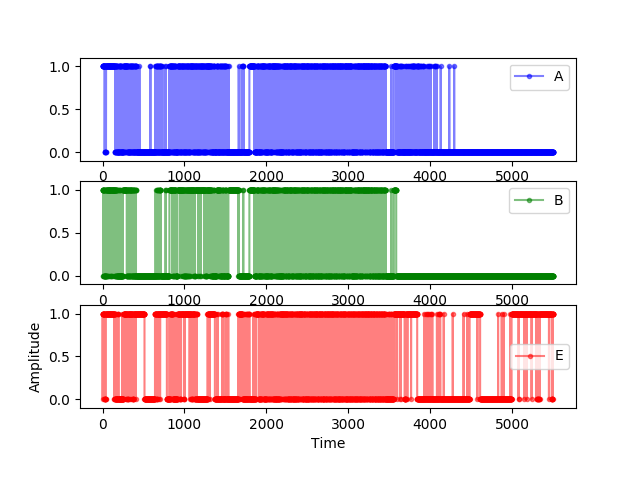
\includegraphics[width=0.65\textwidth ]
		{Bilder/a4-q0-2.png}
		\caption{\textit{quant0}}
		\label{fig:4.1}
\end{figure}


\begin{figure}[hbt!]
	\centering
		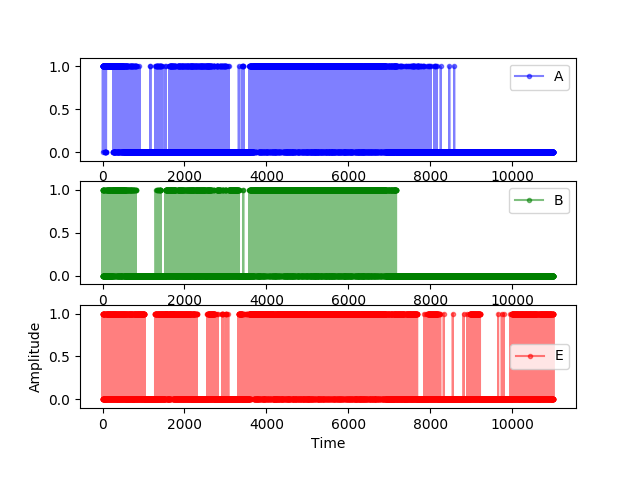
\includegraphics[width=0.65\textwidth ]
		{Bilder/a4-q1-2.png}
		\caption{\textit{quant1}}
		\label{fig:4.2}
\end{figure}


\begin{figure}[hbt!]
	\centering
		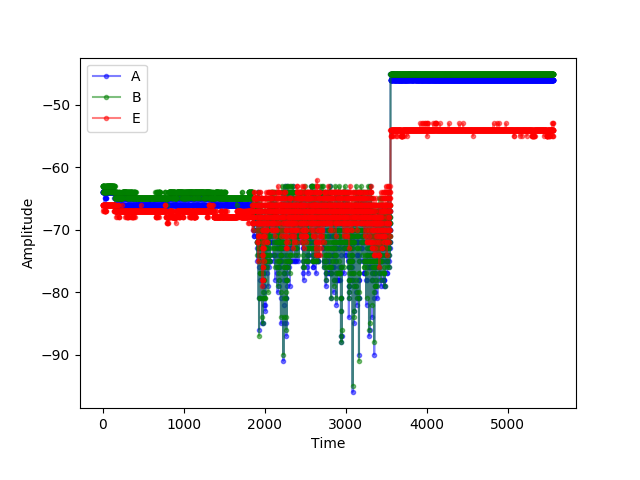
\includegraphics[width=0.65\textwidth ]
		{Bilder/a4-q0-1.png}
		\caption{\textit{Signalstärkenverlauf}}
		\label{fig:4.3}
\end{figure}
Wenn man Abbildung~\ref{fig:4.1} betrachtet, so erkennt man, 
dass Einflüsse wie Bewegung und Distanz eine große Rolle 
spielen.\\
Analysiert man die Unterschiede so wird klar, dass Bewegung
und größere Distanz einen Angreifer benachteiligen.